\chapter{Diseño}
\section[Diagrama de clases]{Diagrama de clases}
En este apartado se mostrarán los diagramas de clases de los elementos más importantes de la aplicación.
\newgeometry{scale=1}
\thispagestyle{empty}
{%
	\label{fig:fragment_diagram}
	\centering
	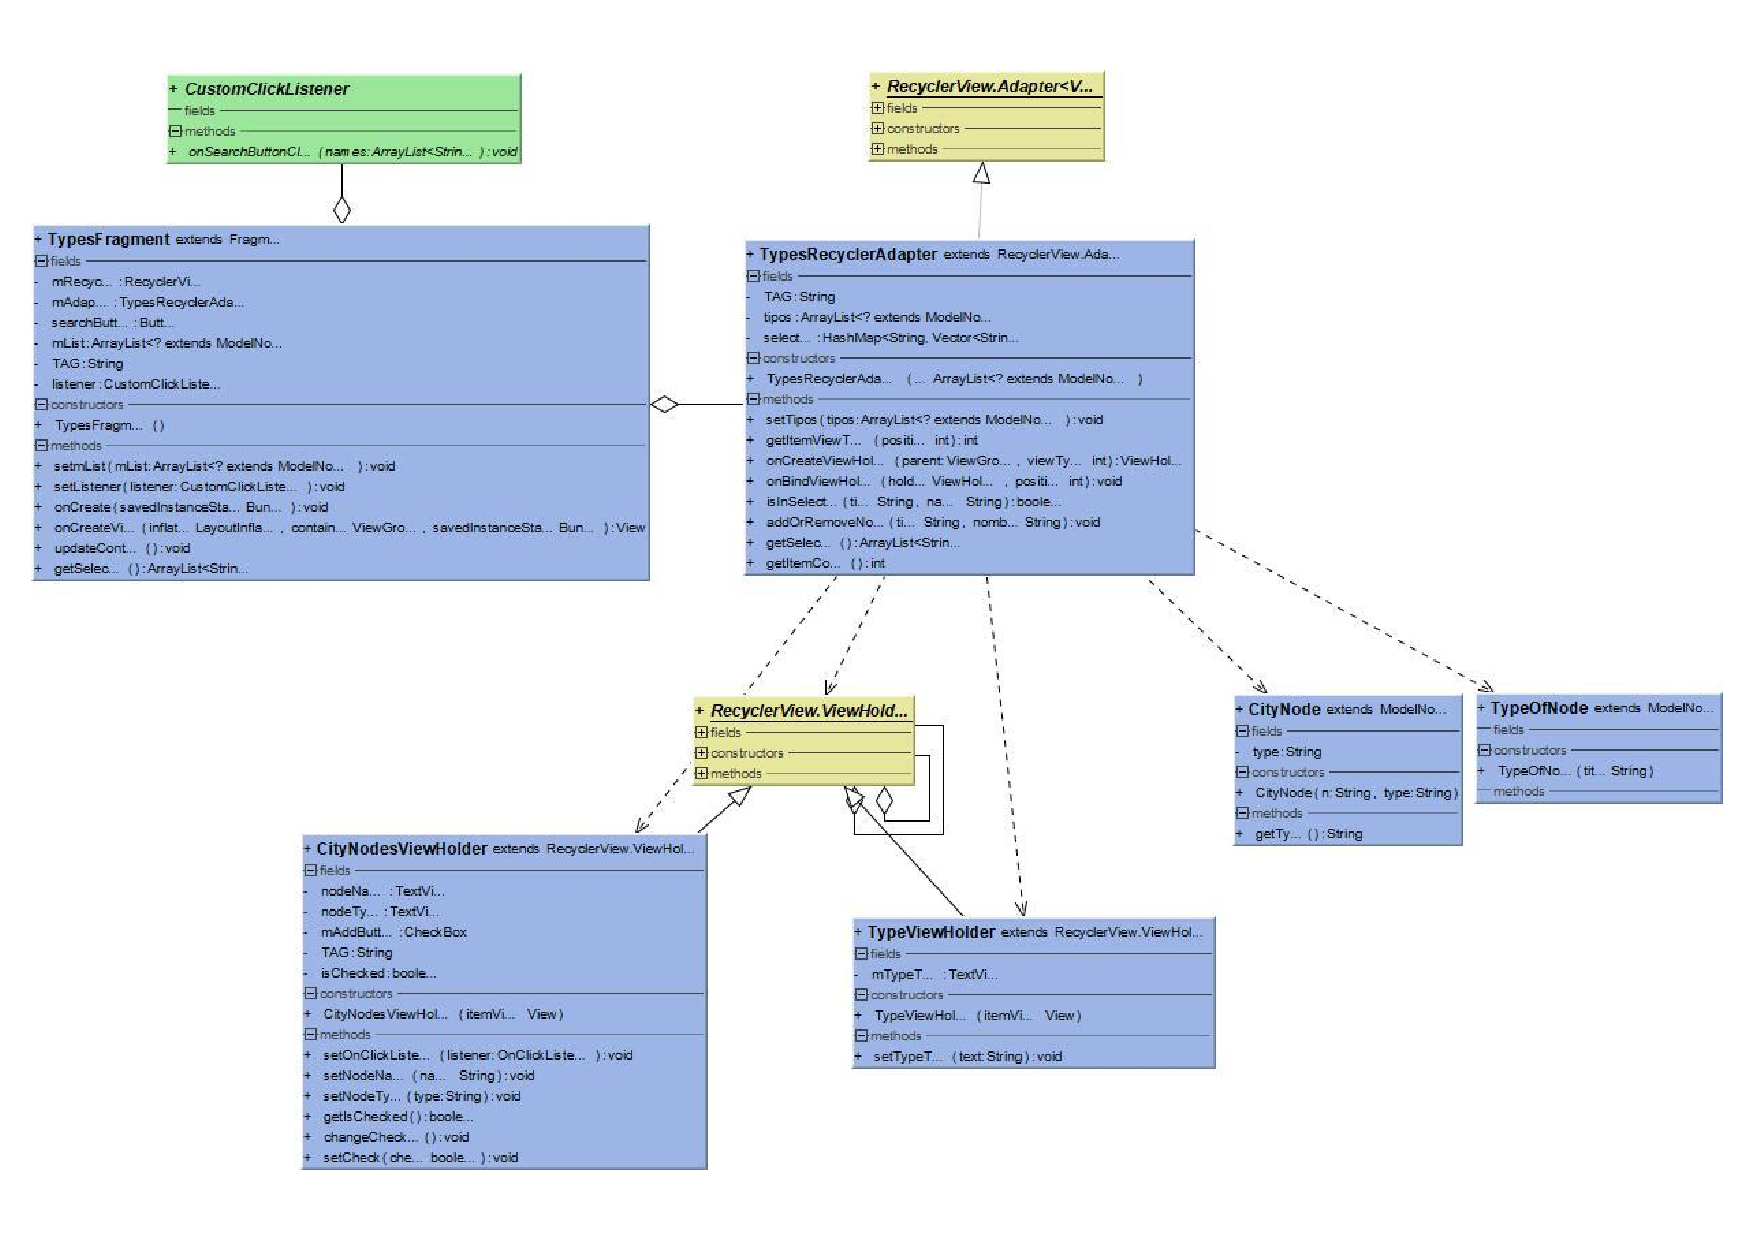
\includegraphics[scale=.95,angle=90]{imagenes/fragment_class_diagram.pdf}
	\captionof{figure}{Diagrama de clases del fragment}
	\par
}
\restoregeometry

\newgeometry{scale=1}
\thispagestyle{empty}
{%
	\label{fig:main_activity_diagram}
	\centering
	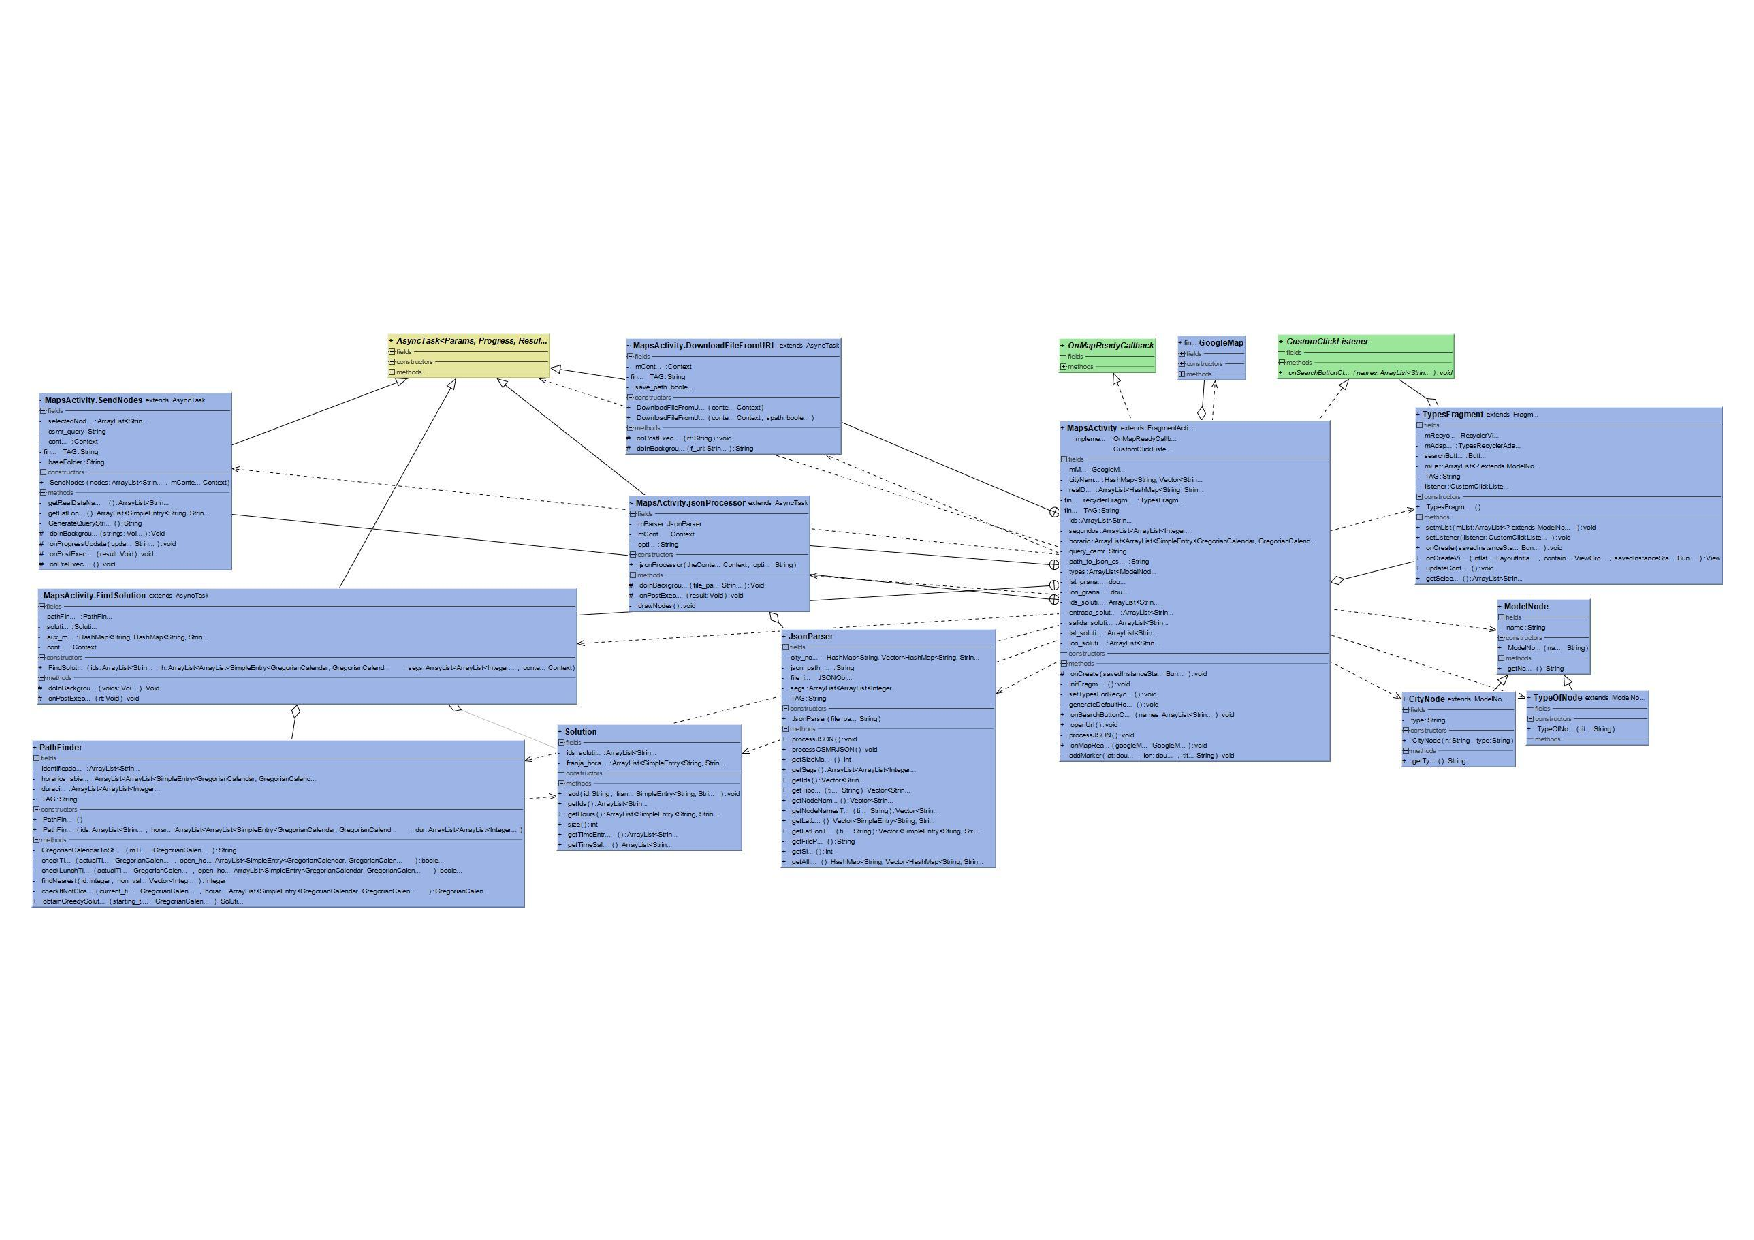
\includegraphics[scale=.95,angle=90]{imagenes/main_activity_class_diagram.pdf}
	\captionof{figure}{Diagrama de clases de la actividad principal}
	\par
}
\restoregeometry

\newgeometry{scale=1}
\thispagestyle{empty}
{%
	\label{fig:models_diagram}
	\centering
	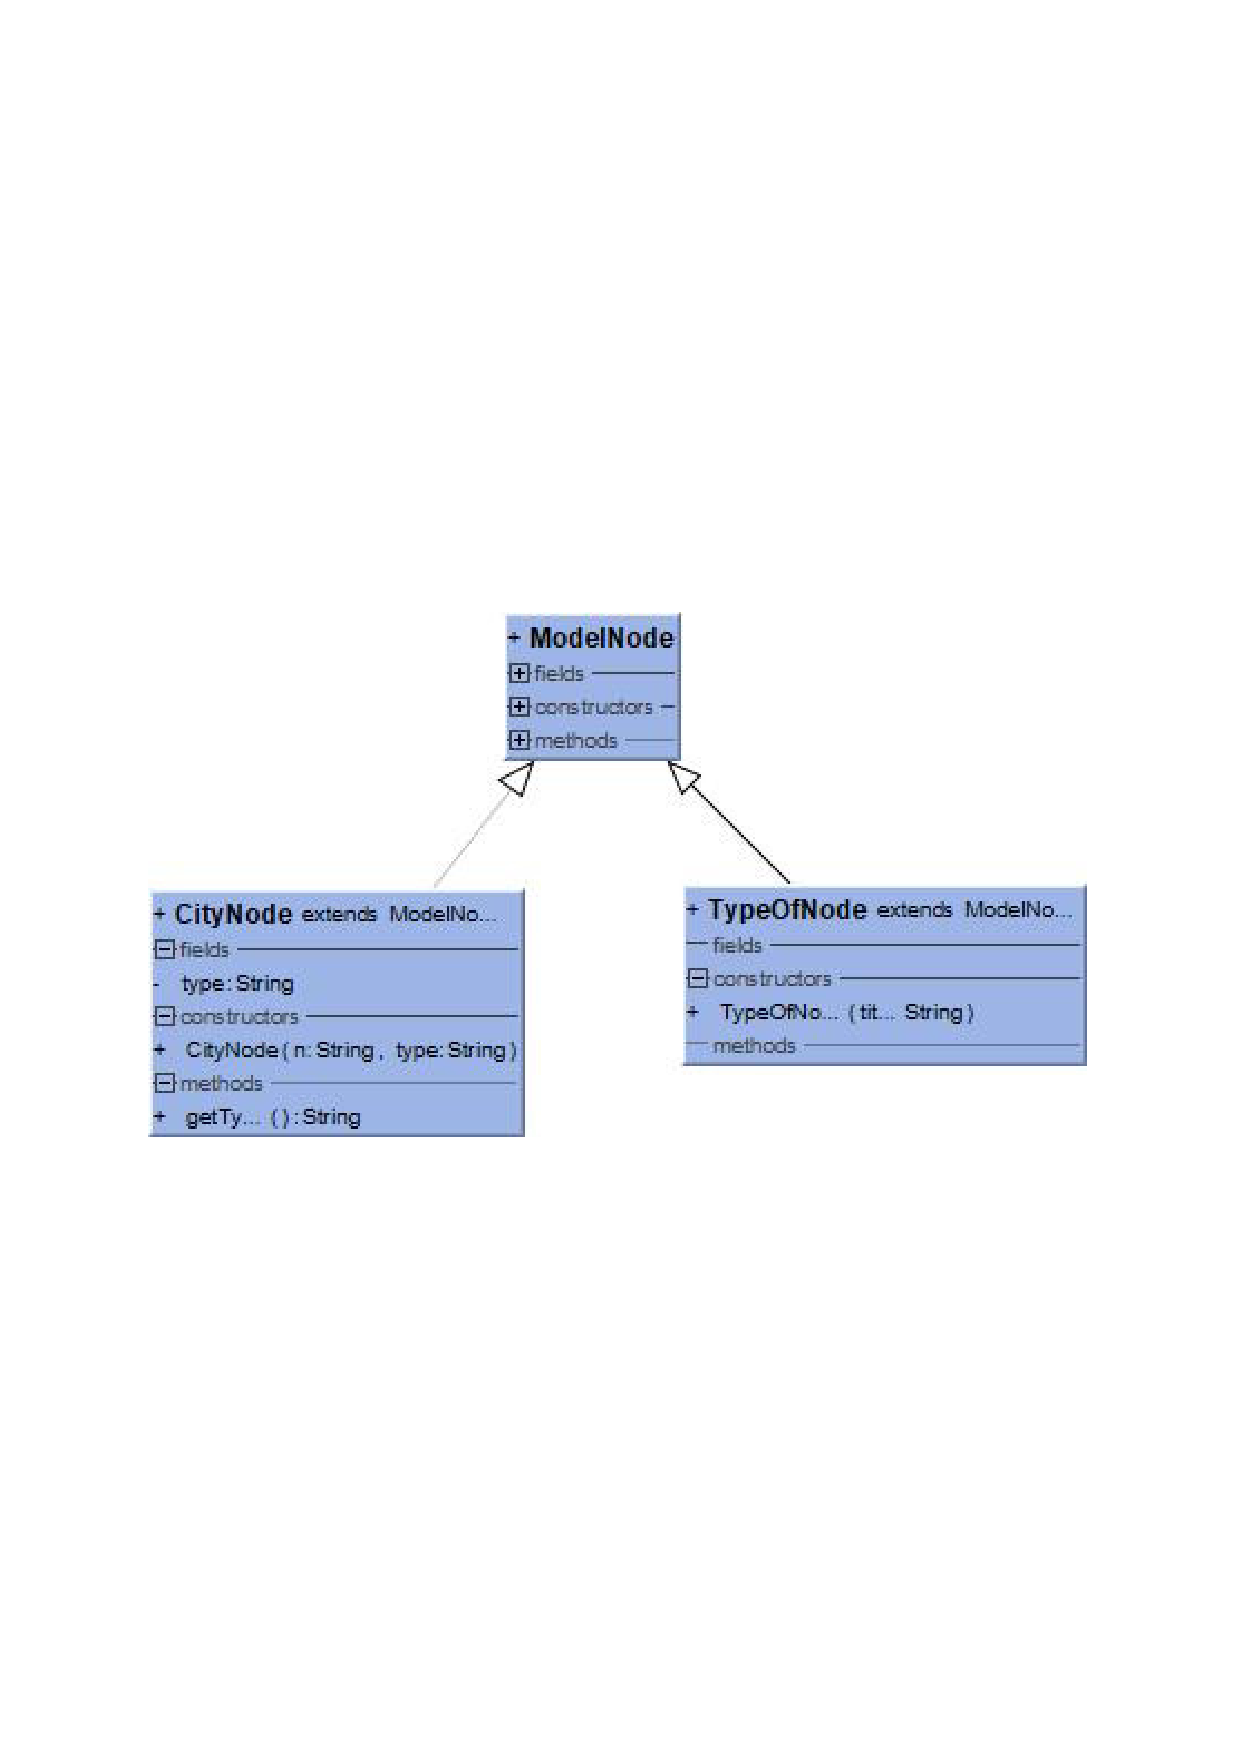
\includegraphics[scale=.95,angle=90]{imagenes/models_class_diagram.pdf}
	\captionof{figure}{Diagrama de clases del paquete models}
	\par
}
\restoregeometry

\newgeometry{scale=1}
\thispagestyle{empty}
{%
	\label{fig:result_activity_diagram}
	\centering
	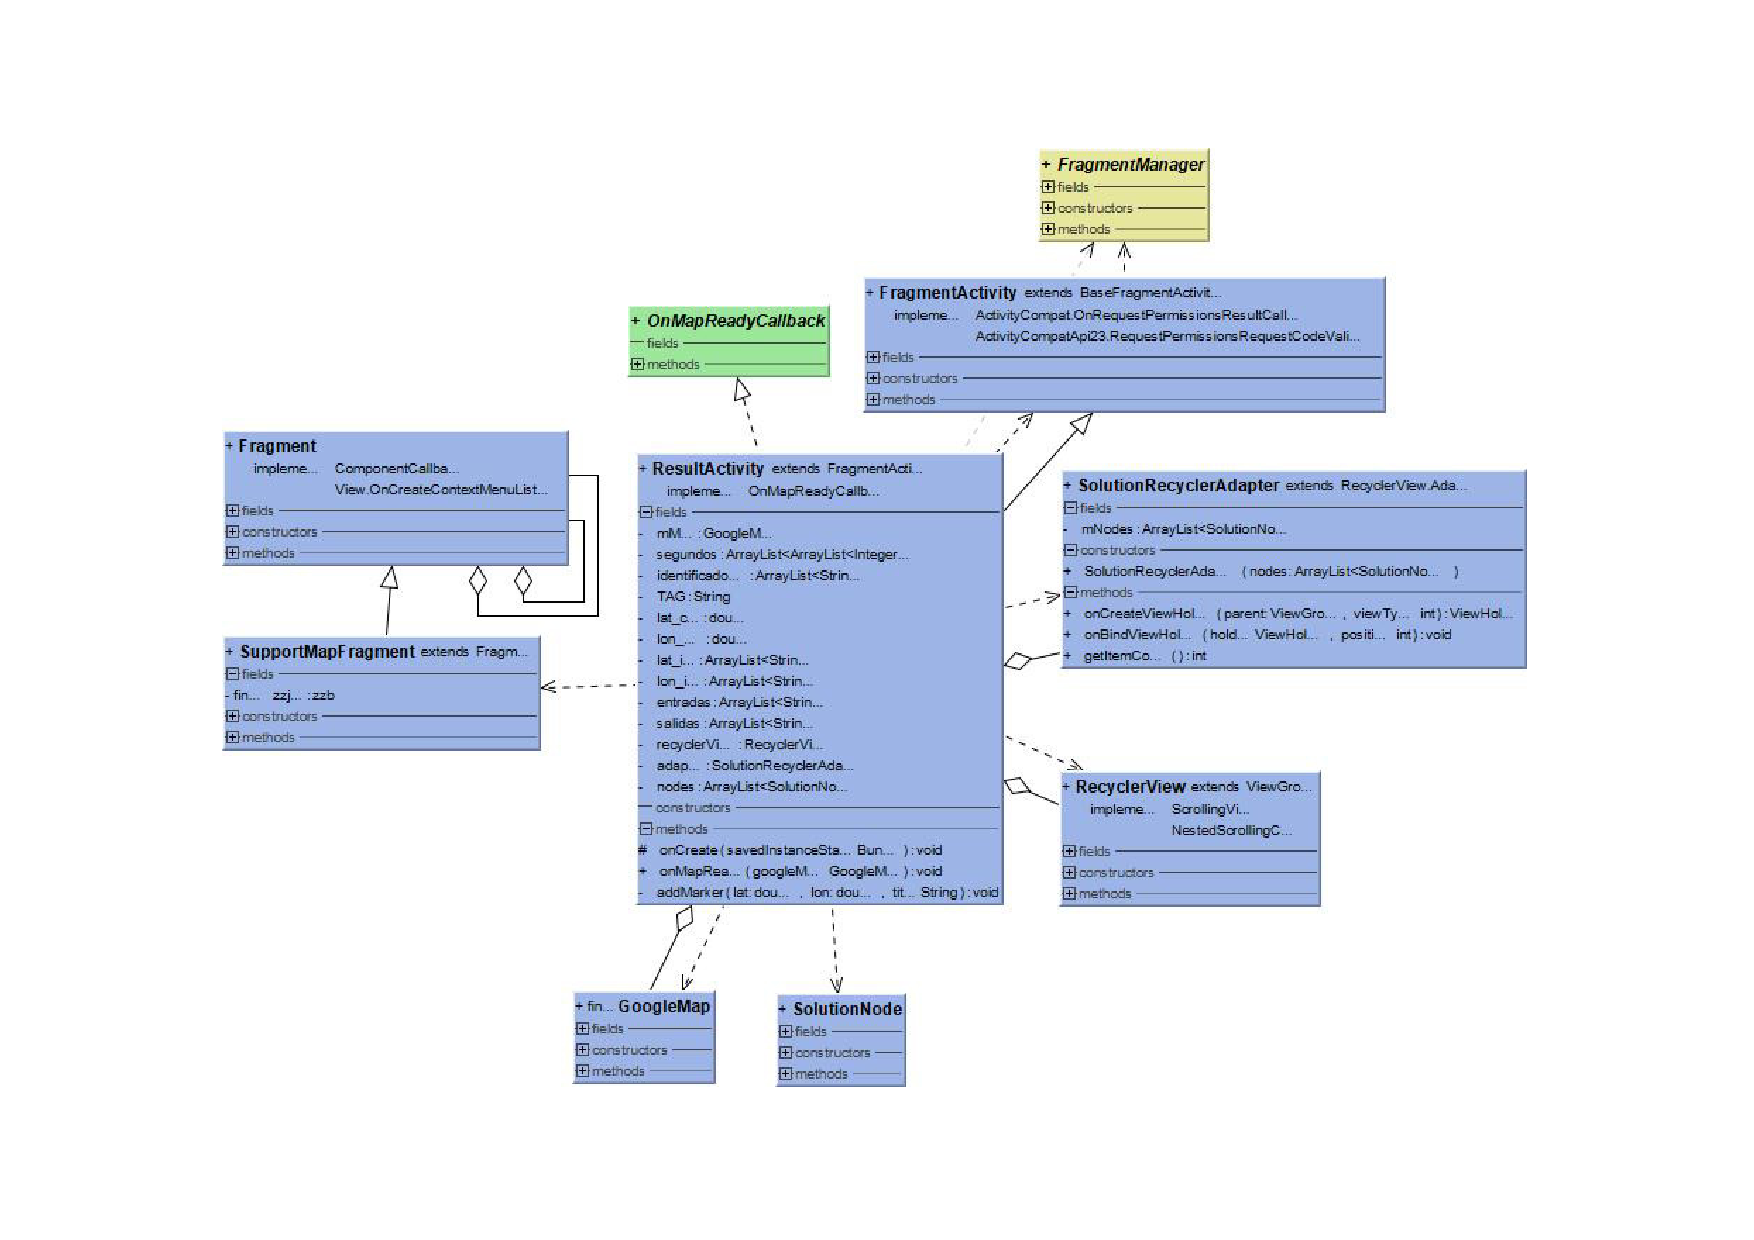
\includegraphics[scale=.95,angle=90]{imagenes/result_activity_class_diagram.pdf}
	\captionof{figure}{Diagrama de clases del activity ResulActivity}
	\par
}
\restoregeometry

\newgeometry{scale=1}
\thispagestyle{empty}
{%
	\label{fig:solution_recycler_diagram}
	\centering
	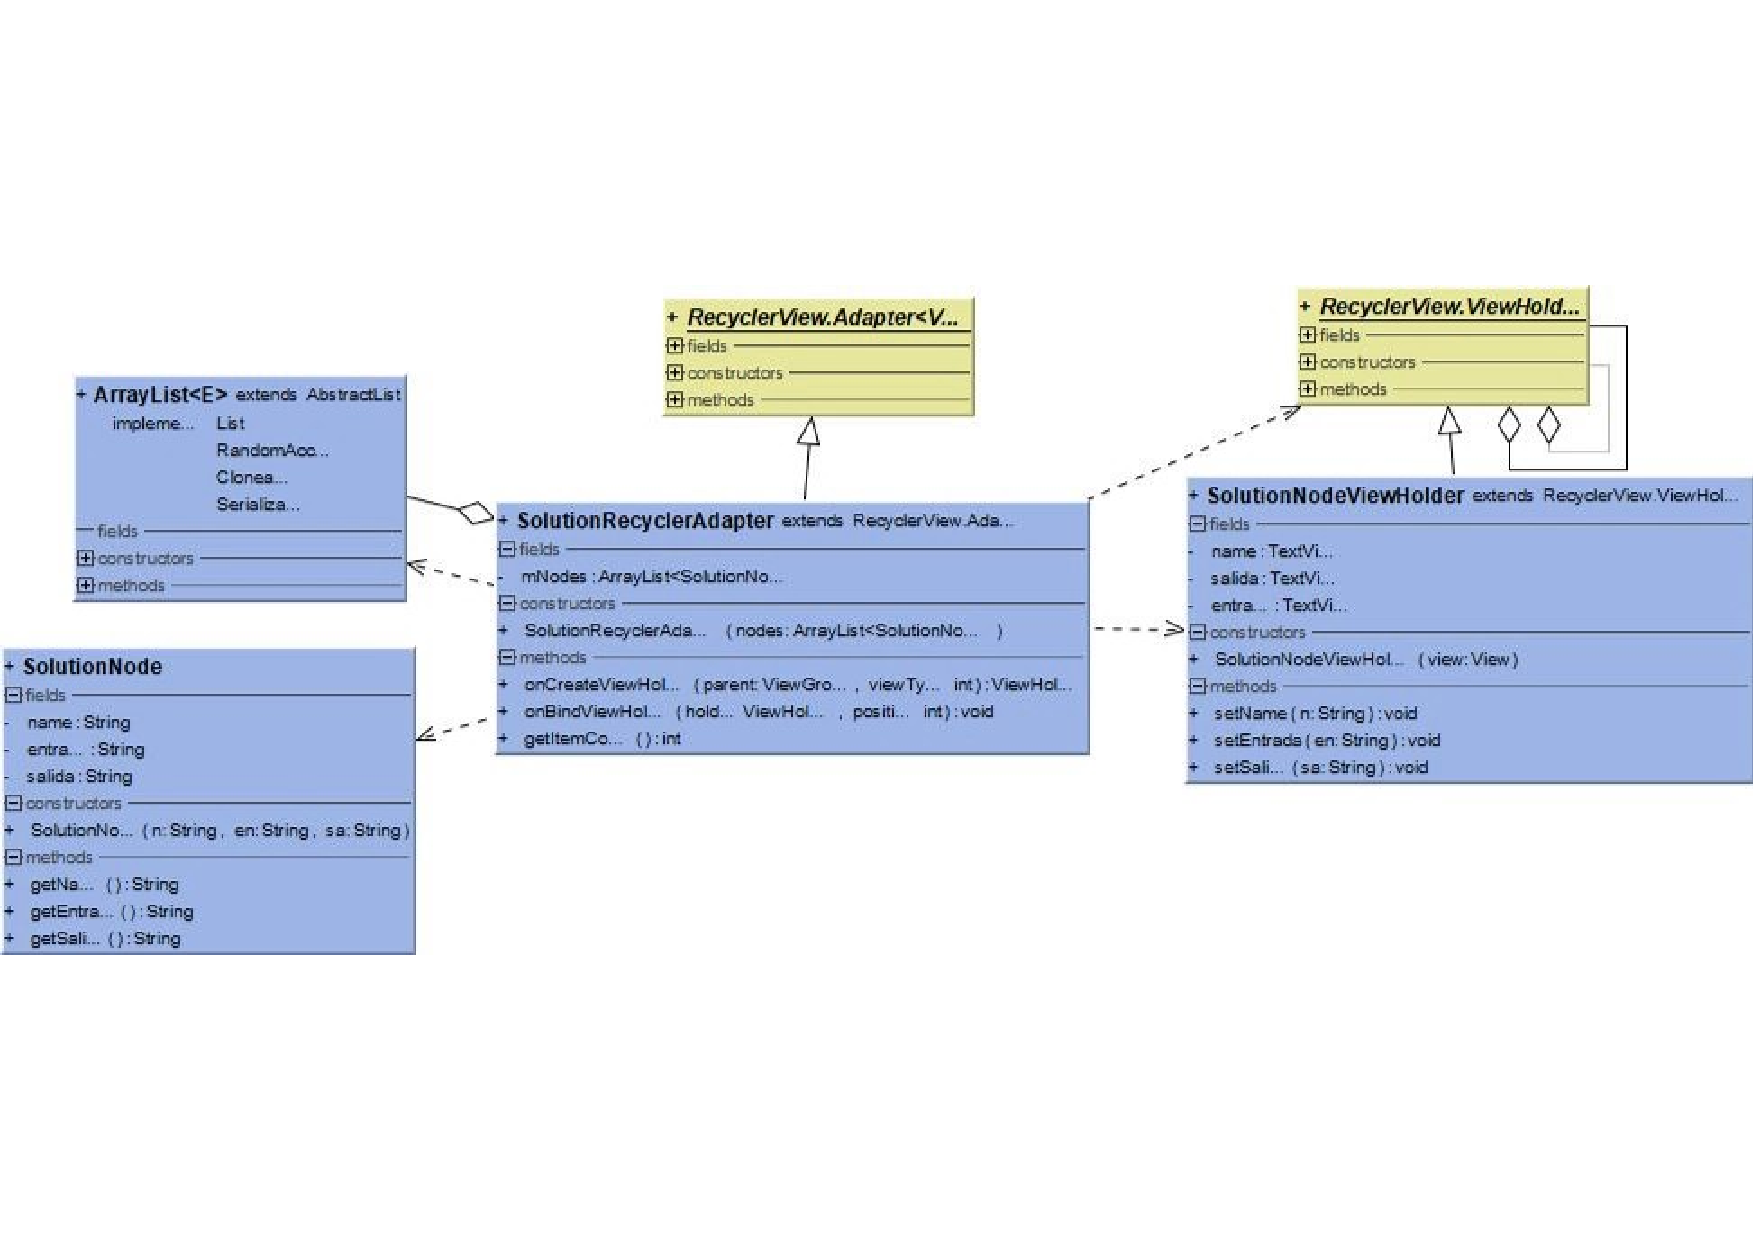
\includegraphics[scale=.95,angle=90]{imagenes/solution_recycler_class_diagram.pdf}
	\captionof{figure}{Diagrama de clases de la clase SolutionRecycler}
	\par
}
\restoregeometry



